\section{Behavior}

Branch predictor works as a memory module that contains past branches information, and uses them to predict new values. There are three memory tables, with 1024 entries. These entries are accessed with the bits 11 to 2 of the program counter of the fetch stage. 

\begin{figure}[h]
\centering
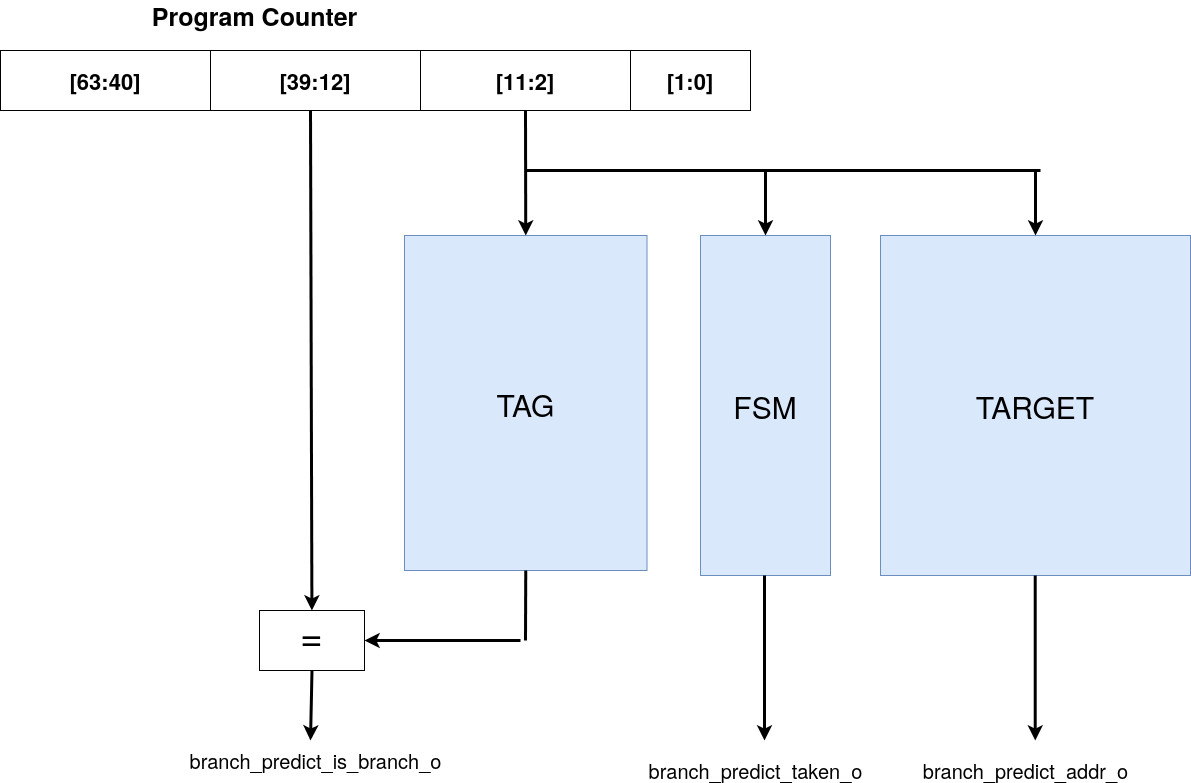
\includegraphics[width=1\linewidth]{branch_predictor.png}
\end{figure}

The first table stores the tags of the branches. A tag is a subset of the bits from 39 to 12 of the PC. We do not store bits 40 to 64 since our processor has support only for 40 bit virtual addresses. Therefore, the table stores 40x1024 bits. The tag read from the table is compared with the equivalent bits of the PC, and if they are equal the BP predicts that the fetched address is a branch. This is done through signal branch\_predict\_is\_branch\_o.

The second table stores the target addresses of the branches, the address where the branches jump to. Again this table stores 1024x40 bits. This address is output to signal bimodal\_predict\_addr\_o and to branch\_predict\_addr\_o. Since this signal is 64 bit long, bits 39 to 63 are filled with zeros.

The third table stores the finite machine state of the branches. This machine consists on a 2-bit saturating counter. Therefore the table stores 1024x2 bits. When the branch prediction is doing predictions it reads the table and uses the counter to predict if the branch will be taken or not. If the upper bit is 0 the branch is not taken (values 0 or 1), and if the upper bit is 1 then the branch is taken (values 2 or 3). The decision is output though signals branch\_predict\_taken\_o and bimodal\_predict\_taken\_o.


In order to make good predictions, the tables must be updated with the latest information of the branches. Therefore, the branch prediction is connected to the output of the ALU. In case a branch arrives to the ALU, signal is\_branch\_EX\_i is set to 1. And signals pc\_execution\_i, branch\_addr\_result\_exec\_i, branch\_taken\_result\_exec\_i are respectively updated with the program counter of the instruction at execution stage, the address the branch should have jump and the result of the branch (taken or not taken).

